\section{Filtrační obvody}
-funkce, příklady realizací, důvody použití v převodnících, aproximační charakteristiky, přesné filtry.

\subsection{Funkce}
Jedná se obvykle o filtry typu dolní propust.
Je určen k:
\begin{itemize}
\item potlačování záznějí (Aliasing) – omezení šířky pásma vstupního signálu,
\item  potlačení kvantovacího šumu na výstupu DAC
\item a potlačení střídavých složek v nepřímých převodnících DA.
\end{itemize}

Problém aliasingu (záznějí) je vidět na obrázku \ref{fig:ali}, kde vstupní analogový signál má kmitočtovou odezvu (\ref{fig:ali}a)) a kmitočet f\textsubscript{b} je maximální kmitočet vstupního signálu. Pokud je vstupní analogový signál vzorkován s vzorkovacím kmitočtem f\textsubscript{s} je kmitočnotá odezva tohoto signálu jako na \ref{fig:ali}b).

Spektrum vstupníhosignálu se zrcadlí na kmitočtu f\textsubscript{s} a každé jeho vyšší harmonické složce. Pokud ale f\textsubscript{b} přesáhne polovinu f\textsubscript{b}, dojde k částečnému překrytí postranních složek, viz \ref{fig:ali}c). V důsledku toho pak může dojít k významné ztrátě informace o původním signálu, který pak již nelze rekonstruovat do původní podoby.

Proto musí být dodržen vzorkovací teorém:
\begin{equation}
 f_{s} > 2*f_{b}
\end{equation}

Uvedený vztah platí pouze pro harmonický signál resp. nejvyšší harmonickou složku jiného signálu. Antialiasingový filtr je použit proto, aby zabránil překrytí postranních složek, \ref{fig:ali}d)

   \begin{figure}[h]
   \begin{center}
     \includegraphics[scale=0.6]{images/Aliasing.png}
   \end{center}
   \caption{Problém aliasingu}
   \label{fig:ali}
  \end{figure}
\pagebreak  
\subsection{Příklady realizací}
Klasické aktivní filtry se k výše uvedeným účelům užívají stále méně z důvodu složitého seřizování, obtížně se přelaďují a nejsou příliš vhodné k integraci na čip. Proto se používají filtry využívající techniku spínaných kapacitorů (SC). Hlavním důvodem využití této techniky byla jednoznačně možnost nahrazení pasivního prvku – rezistoru, který na čipu zabírá velkou plochu, kapacitorem a spínačem MOS, které simulují funkci rezistoru
   \begin{figure}[h]
   \begin{center}
     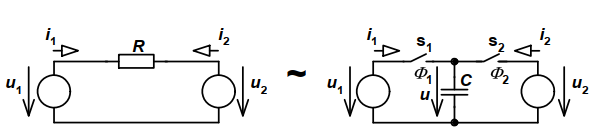
\includegraphics[scale=0.6]{images/SC.png}
   \end{center}
   \caption{Princip SC}
  \end{figure}
  
\begin{equation}
i=\frac{u}{R} \approx i_{ekv}=\frac{q}{T}=\frac{C*u}{T}=\frac{u}{R_{ekv}} => R_{ekv}=\frac{T}{C}
\label{eqn:i}
\end{equation}  

kde R je odpor, C je kapacita a T časová konstanta, q je náboj na kapacitoru, i\textsubscript{ekc} je celkový proud tekoucí
kapacitorem a u je celkové napětí na kapacitoru.

Rezistor, kterým protéká kontinuálně konstantní proud I lze nahradit spínačem s rezistorem. Z tohoto yplývá, že proud tekoucí kapacitorem má impulzní charakter (Obrázek \ref{fig:impulz}), tedy naprosto jiný, než je tomu u rezistoru. Pokud ale budeme uvažovat střední hodnotu těchto impulzů, která bude odpovídat rov. \ref{eqn:i}), je možné uvedené obvodové prvky nahradit.

   \begin{figure}[h]
   \begin{center}
     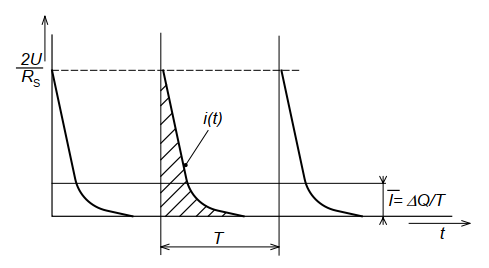
\includegraphics[scale=0.6]{images/Impulz.png}
   \end{center}
   \caption{Impulzní průběh SC}
   \label{fig:impulz}
  \end{figure}
  
  
\textbf{Z této náhrady vyplynulo několik výhod:} 
\begin{itemize}
\item na rozdíl od rezistoru, jehož výrobní chyba v IO je 5 až 20 \%, je přesnost
zpracování vstupního analogového signálu dána pouze přesností poměru kapacit,
která může být řádově až 0,01 \%,
\item  kapacitory je možné v technologii CMOS snadněji implementovat na čip,
\item  spínače CMOS mají v sepnutém stavu nízký odpor (řádu desítek ohmů),
\item  dobrá přesnost časových konstant,
\item  dobrá napěťová linearita
\item a dobré teplotní charakteristiky.
\end{itemize}

\textbf{Mezi nevýhody techniky SC patří} 
\begin{itemize}
\item pronikání řídicího hodinového signálu přes spínače do signálové cesty –
dochází ke znehodnocení zpracovávaného užitečného signálu,
\item injekce náboje ze spínače – dochází ke znehodnocení zpracovávaného
užitečného signálu,
\item  jednotlivé fáze řídicího hodinového signálu musí být realizovány jako
nepřekrývající se, což klade vysoké nároky na přesnost generovaného řídicího
hodinového signálu (viz. Obrázek \ref{fig:sig}),
\item chyby přizpůsobení použitých kapacitorů – negativně ovlivňují přesnost
převodu
\item a parazitní kapacity.
\end{itemize}
   \begin{figure}[h]
   \begin{center}
     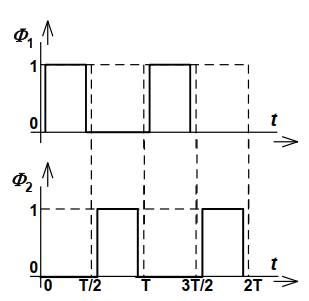
\includegraphics[scale=0.6]{images/SC_sig.png}
   \end{center}
   \caption{Řidicí a nepřekrývající se hodinové signály}
   \label{fig:sig}
  \end{figure}
\pagebreak
\subsubsection{Stejnosměrné přesné filtry}
Jsou vhodné jako antialiasingové filtry i jako filtry pro nepřímé převodníky. Kaskádní struktura filtru, však není pro realizaci příliš vhodná, protože se uplatňuje napěťová nesymetrie použitých OZ ve výstupním signálu. Jistým řešením je použití pasivních prvků, což způsobuje problémy při realizaci induktorů. Východiskem je tedy použití nekaskádní struktury aktivního filtru.

   \begin{figure}[h]
   \begin{center}
     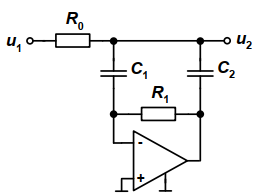
\includegraphics[scale=0.8]{images/Nekas.png}
   \end{center}
   \caption{Nekaskádní zapojení aktivního filtru 2. řádu}
   \label{fig:nekas}
  \end{figure}

\subsection{Důvody použití v převodnících}  
Plní hned několik funkcí, mezi které patří zejména potlačení aliasingu (záznějí), potlačení kvantovacího šumu na výstupu DAC a potlačení střídavých složek v nepřímých převodnících DA.
\subsection{Aproximační charakteristiky}

Filtry obecně nejsou specifikovány pouze mezními kmitočty, které definují propustné a zádržné oblasti. Důležitá je také zvolená aproximační metoda realizace filtru. V případě filtrů typu dolní propust existují čtyři základní aproximace, a to aproximace podle Butterwortha, Chebysheva (vč. inverzní verze) a Cauera (Darlingtona).

\textbf{Butterworthova aproximace} má maximálně plochou kmitočtovou charakteristiku kolem počátku a monotónně klesající průběh od mezního kmitočtu v nepropustném pásmu.

\textbf{Aproximace podle Chebysheva} je v propustném pásmu mírně zvlněná s monotónně klesající průběhem od mezního kmitočtu v nepropustném pásmu. 

\textbf{Inverzní Chebyshevova aproximace} má maximálně plochou kmitočtovou charakteristiku v propustném pásmu a pásmu potlačení je mírně zvlněná. 

\textbf{Aproximace Cauerova nebo také Darlingtonova} je mírně zvlněná v obou pásmech své kmitočtové charakteristiky. Proto se také pro ni ustálil výraz eleptický filtr.

   \begin{figure}[h]
   \begin{center}
     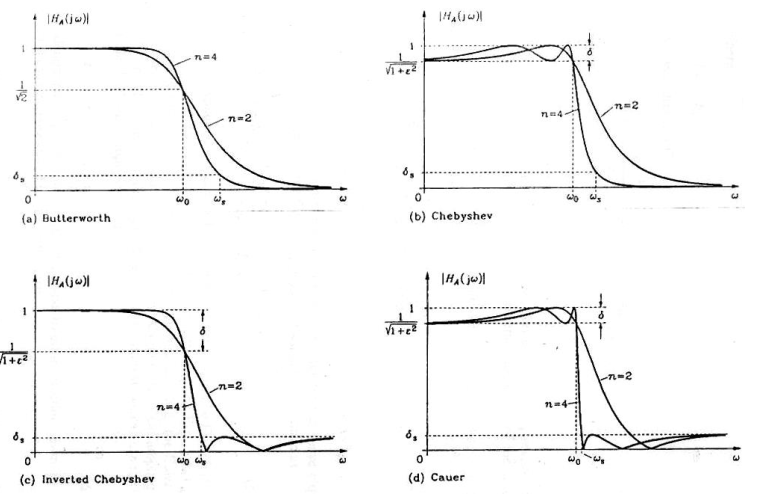
\includegraphics[scale=0.8]{images/Aprox.png}
   \end{center}
   \caption{Jednotlivé aproximace}
   \label{fig:sig}
  \end{figure}
\newpage 
\subsection{Přesné filtry}    
  Realizace filtru – ss přesné filtry
\begin{itemize}
\item výhodou těchto struktur je stejnosměrné oddělení všech
výstupů OZ pomocí kapacitorů od hlavní signálové cesty,
\item šum OZ se uplatňuje tím více, čím jsou blíže hlavní signálové
cesty => horní OZ nízkošumové,
\item filtr nesmí být zatěžován =>doplnit na výstupy vysoce kvalitní
oddělovací zesilovač.
\end{itemize}
Viz. Obrázek \ref{fig:nekas}.






